\chapter{Lexer}
In this chapter the requirements of the lexer for NISSE will be presented, along with a listing of the tokens for NISSE.
\section{Requirements}
The requirements for the lexer are:
\begin{itemize}
		\item The lexer should be able to take any plain text file as input.
		\item The lexer should be able to recognize the input and make tokens according to the token list for NISSE.
		\item The lexer should be able to output meaningful error messages when it cannot match the input to any token.
		\item The lexer should be able to output tokens so that the parser can use them.
\end{itemize}

\newpage
\section{Token List}
In order to create the syntax in chapter \ref{SSyntax}, tokens have to be identified for later use.
\\ \\
The tokens for the language is listed in listing \ref{lst:Lexer}.

\begin{lstlisting}[frame=single, caption={Token List of NISSE in EBNF.}, label=lst:Lexer]
char            = ? [a-�A-�]+ ? ;
digit           = ? [0-9]+ ? ;
underscore      = '_' ;
hyphen          = '-' ;
dotv1           = '.' ;
commav1         = ',' ;
space           = ' ' | '	';
atsign          = '@' ;
lcurly          = '{' ;
rcurly          = '}' ;
pipe            = '|' ;
fslash          = '/' ;
bslash          = '\' ;
colon           = ':' ;
scolon          = ';' ;
blist           = '*' ;
nlist           = '#' ;
percent         = '%\%%' ;
exclamation     = '!' ;
eolv1           = \r | \n | \r\n ;
format_kwd      = '@u' | '@b' | '@i' | '@apply' | '@image' | '@title' | '@subtitle';
setting_kwd     = '@setting' ;
begin_kwd       = '@begin' ;
end_kwd         = '@end' ;
url             = '@url' ;
\end{lstlisting}
\begin{table}
\begin{center}
\begin{tabular}{|l|l|}
\hline 
Usage & Notation \\ 
\hline 
definition & = \\ 
\hline 
termination & ; \\ 
\hline 
alternation & | \\ 
\hline 
option & [ ... ] \\ 
\hline 
repetition & \{ ... \} \\ 
\hline 
grouping & ( ... ) \\ 
\hline 
terminal string & ' ... ' \\ 
\hline 
comment & (* ... *) \\ 
\hline 
special sequence & ? ... ? \\ 
\hline 
\end{tabular}
\caption{EBNF syntax}
\label{tbl:EBNFSyntax}
\end{center}
\end{table}
An example is the line \lstinline!S = a {b}+ [ {c}+ ] ( a | b ) ;! that translates to \lstinline!S = a!, followed by at least one \lstinline!b!, followed by none or at least one \lstinline!c!, followed by \lstinline!a! or \lstinline!b!. The special sequence is used for writing anything that is not directly an EBNF, defined in \ref{tbl:EBNFSyntax}. An example is \lstinline!char = ? a-�A-� ? ;! in listing \ref{lst:Lexer} where all letters from a to z is defined using both capital and non-capital. \\
\noindent{The abnormal in this token list is \lstinline!format{\_}kwd!, \lstinline!setting{\_}kwd!, \lstinline!begin{\_}kwd! and \lstinline!end{\_}kwd!, (kwd is short for ``keyword''). These keywords are explicit, because in the productions in which they occur they can only be on the left hand side of a left curly bracket. Their specific use is explained in chapter \ref{SSyntax}.}
\\ \\
The reason each expression has its own token and not a general production, is to easily see the difference between the special tokens and the normal ones, without the need to check that a given token in the syntax analyser is the right token.
\\ \\ 
\lstinline!Char! is used whenever characters needs to be used in the code. \lstinline!Char! is used both for plain text and identifiers. \\
\lstinline!Digit! is used whenever numbers need to be used in the code. \\

\subsection{NFA}
Figure \ref{fig:nfaer} is a NFA (Nondeterministic Finite Automaton) for when the user inserts an \texttt{atsign}, which can become a lot of different tokens. It will always take an input before an epsilon\footnote{The empty set.}, for instance, if an \texttt{atsign} and an \texttt{i} is written, it looks at the next tokens, before it uses the epsilon transition.

\begin{figure}[h!]
	\centering
		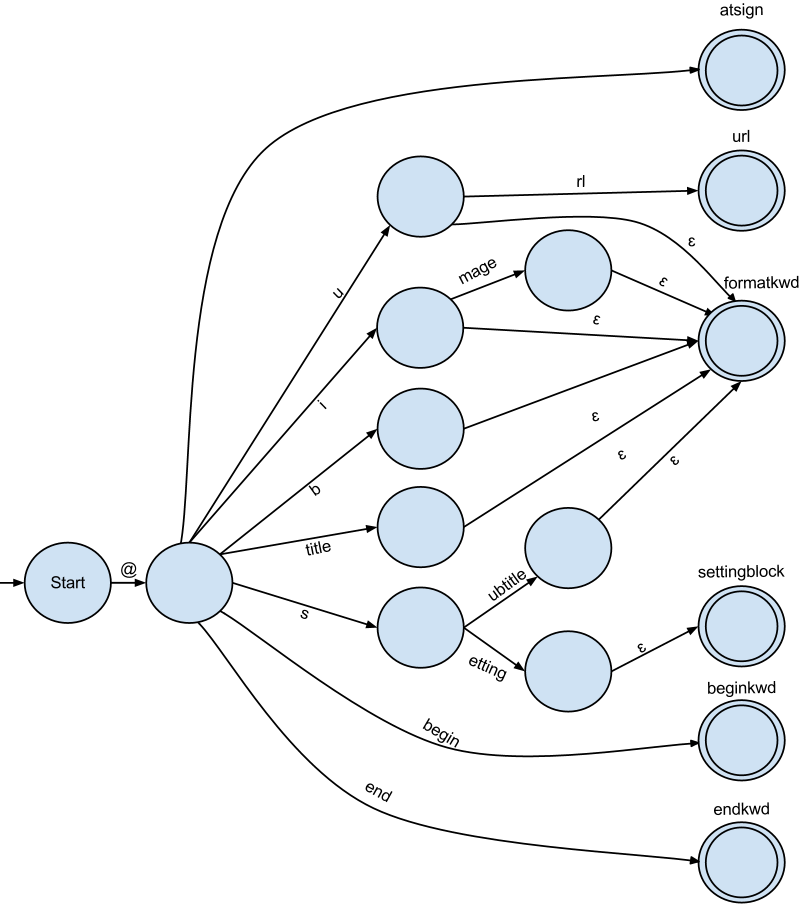
\includegraphics[width=1\textwidth]{./images/nfaer.png}
	\caption{NFA for \texttt{atsign}}
	\label{fig:nfaer}
\end{figure}

\noindent{The \texttt{atsign} can create a number of different tokens, shown in figure \ref{fig:nfaer}, these are; \texttt{formatkwd, settingblock, beginkwd, endkwd, url} and if the text does not match any of these, it is tokenized as an \texttt{atsign} and the text after the \texttt{atsign} is tokenized as a another token.}

\subsubsection*{Regular expression}
The regular expression for figure \ref{fig:nfaer} is shown in listing \ref{lst:Regularexpression}
\begin{lstlisting}[frame=single, caption=Regular expression, label=lst:Regularexpression]
%$@ ( (i (\epsilon \cup mage)) \cup (u ( \epsilon \cup rl)) \cup (b( \epsilon \cup egin) ) \cup title \cup (s(ubtitle \cup etting)) \cup end \cup \epsilon)$%
\end{lstlisting}